\chapter{Étude de l'existant}

\section{Analyse des algorithmes et méthodes existantes}
La génération procédurale de terrains étant un sujet qui intéresse de nombreux développeurs, il existe un nombre très importants d'algorithmes dans ce domaine. Nous en avons sélectionné une dizaine qui pourront nous \^etre utiles pour ce projet. Nous pouvons les catégoriser de la façon suivante :
\begin{itemize}
\item les bruits ;
\item les fractales ;
\item les raffinements.
\end{itemize}


\subsection{Les bruits}
Un bruit est une application de $\mathbb R^n$ dans $\mathbb R$, on lui fourni
une entrée sur n-dimensions avec coordonnées réelles et il retourne un réel.
Un bruit permet donc d'associer une valeur à chaque point de l'espace.\\

Les bruits dit cohérents possèdent les trois propriétés suivantes :
\begin{itemize}
\item la même valeur d'entrée retournera toujours la même valeur de sortie ;
\item un petit changement dans la valeur d'entrée produira un petit changement dans la valeur de sortie ;
\item un grand changement dans la valeur d'entrée produira un grand changement
dans la valeurs de sortie.\\
\end{itemize}

On peut donc se servir des bruits cohérents pour générer des textures ou
bien des cartes d'élévations, pour cela on fourni en entrée au bruit les
coordonnées de chaque point de la texture ou de la carte d'élévation
et la sortie nous donne la couleur ou l'élévation.\\
Nous allons maintenant présenter les algorithmes des bruits de cellule, de valeur, de Perlin et de simplexe.

\subsubsection{Bruit de cellule}
Le bruit de cellule propose une représentation différente des points dans l'espace. Effectivement, ils sont caractérisés par les points autour d'eux.
Cela signifie qu'un point existant proche du point traité aura plus d'influence sur la valeur de ce dernier.
\paragraph{}
La première étape consiste donc à placer les points existants. Ils sont générés sur une grille 2D de façon pseudo-aléatoire et chaque case de la grille peut contenir un ou plusieurs points (comme illustré dans la figure~\ref{fig:cell-noise}).
La seconde étape est d'intégrer chaque point à traiter sur cette grille puis de comparer la distance entre le point à traiter et ses plus proches voisins.

\begin{figure}[ht!]
    \begin{center}
        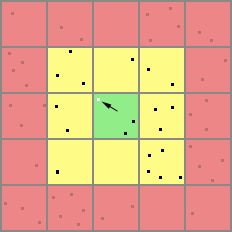
\includegraphics[width=10cm]{resources/cellgrid.png}
        \caption{Grille du bruit de cellule}
        \label{fig:cell-noise}
    \end{center}
\end{figure}

L'élévation du point traité sera donc le résultat du calcul de distance.
\paragraph{}
Il est possible d'obtenir divers résultats selon la méthode de calcul de distances utilisées. Effectivement, il existe plusieurs méthodes valables pour cet algorithme :
\begin{itemize}
 \item Euclidienne
 \begin{equation}
  distance = \sqrt{(x1 - x2)^2 + (y1 - y2)^2}
 \end{equation}
 \item Manhattan
 \begin{equation}
  distance = abs(x1-x2) + abs(y1-y2) 
 \end{equation}
 \item Chebyshev
 \[
    distance= 
\begin{cases}
    |x1-x2|,& \text{si } |y1-y2|\geq|x1-x2|\\
    |y1-y2|,& \text{sinon}
\end{cases}
\]
 \item Quadratique
  \begin{equation}
  distance = (x1-x2)*(x1-x2) + (x1-x2)*(y1-y2) + (y1-y2)*(y1-y2)
  \end{equation}
\end{itemize}

\paragraph{}
L'algorithme prend donc en entrée :
\begin{itemize}
 \item un point à traiter;
 \item une grille 2D;
 \item une méthode de calcul de distances entre points.
\end{itemize}
L'algorithme retourne une valeur caractéristique de la hauteur du point traité.\newline
Plus de détails concernant ce bruit peuvent être trouvés dans ce livre\cite{Eber02}.


\subsubsection{Bruit de valeur}
Le bruit de valeur (value noise), décrit dans le livre
\cite{Eber02} p.70, est généré à partir de 2 choses :\\
\begin{itemize}
\item un générateur pseudo-aléatoire (c'est à dire un générateur qui semble
aléatoire mais qui lorsque on lui donne la même entrée produit toujours la même
sortie) ;
\item une fonction d'interpolation.\\
\end{itemize}

Le générateur pseudo-aléatoire est une fonction discrète, cette fonction
n'est définie que pour les valeurs entières.

\'Etant donné un nombre pseudo-aléatoire pour chaque coordonnée entière d'un
ensemble à n-dimensions, un bruit de valeur peut-être calculé en interpolant les
valeurs entre chacune de ces coordonnées, obtenant ainsi une application
de $\mathbb R^n$ dans $\mathbb R$.

Si l'on prend l'exemple du bruit de valeur sur une dimension, avec le
générateur pseudo-aléatoire, on obtient une valeur pour chaque coordonnée
entière sur l'axe des X, donc une fonction définie sur $\mathbb N$.
Ensuite, on interpole les valeurs entre chaque entier pour définir une nouvelle fonction prenant en paramètres
un réel. L'interpolation nous permet donc de passer d'une fonction définie sur
$\mathbb N$ à une fonction définie sur $\mathbb R$. La fonction ainsi obtenu
est notre bruit de valeur (voir exemple sur les figures ~\ref{fig:noise_function} et ~\ref{fig:noise_function2}).

\begin{figure}[htp]
  \centering
  \subfloat[Valeurs aléatoires pour chaque point de coordonnée entière.] {
        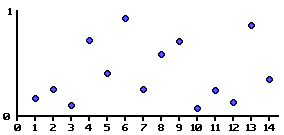
\includegraphics[width=8cm]{resources/noise-function.png}
        \label{fig:noise_function}
  }
  \subfloat[Bruit de valeur généré en interpolant les points.] {
        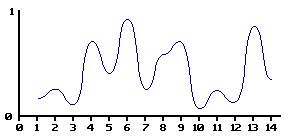
\includegraphics[width=8cm]{resources/noise-function2.png}
        \label{fig:noise_function2}
  }
  \caption{Bruit de valeur sur une dimension (images provenant de
    \cite{PerlinWeb}).}
\end{figure}

Il est possible d'utiliser un grand nombre de fonctions d'interpolations
(linéaire, cosinusoidale, cubique, etc) avec, pour chacune, des rendus
différents (pour un rendu cohérent et détaillé, il est préférable d'utiliser des
valeurs issues d'une interpolation cubique).

\subsubsection{Bruit de Perlin}
Le bruit de Perlin ou bruit gradient ressemble au bruit de valeur mais
diffère par le fait qu'au lieu d'utiliser des nombre pseudo-aléatoire pour chaque
coordonnée entière, on utilise des vecteurs de gradient.

Du fait de sa complexité il ne sera pas décrit de façon détaillée dans ce document.

Pour plus d'information, se référer au livre \cite{Eber02} p.72.

La bibliothèque Libnoise (que nous présenterons dans la section \ref{ref:libnoise} à la page \pageref{ref:libnoise}) propose une implémentation en C++ du bruit de Perlin.

\subsubsection{Bruit de simplexe}
Le bruit de simplexe (simplex noise) est une amélioration faite par Ken Perlin
du bruit de Perlin originale.
Il a, entre autre, l'avantage d'être moins coûteux en complexité pour des dimensions supérieures à trois.

Du fait de sa complexité il ne sera pas décrit de façon détaillé dans ce document.

Pour plus d'informations, se référer à l'article de Gustavson ~\cite{SimplexNoise}
qui décrit précisément le fonctionnement de ce bruit.

\subsubsection{Amplitude et fréquence}
Pour simplifier les explications, nous avons supposé, dans les sections précédentes, que les générateurs
pseudo-aléatoire nous fournissait une valeur pour chaque coordonnée entière,
or dans la réalité la distance entre chaque valeur définie par ces générateur
est définie par l'utilisateur, c'est ce que l'on appelle le \emph{pas}.

La fréquence d'un bruit est définie par $1 / pas$.\\

De plus pour chaque générateur pseudo-aléatoire, la différence entre la
valeur maximum et la valeur minimum possible en sortie nous permet de définir
\emph{l'amplitude} de notre bruit.\\

 Pour chaque bruit \emph{l'amplitude} et la \emph{fréquence} désirés
peuvent donc être spécifiés par l'utilisateur permettant ainsi d'obtenir des
bruits différents selon le résultat attendu.\\

La figure ~\ref{fig:noise-freq-ampl} illustre \emph{l'amplitude} et le \emph{pas}
(wavelength) d'une fonction de bruit.\\

\begin{figure}[ht]
  \centering
  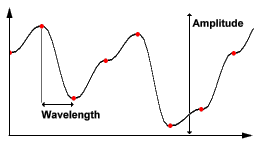
\includegraphics{resources/noise-freq-ampl.png}
  \caption{Fréquence et amplitude d'une fonction de bruit (image provenant de
    \cite{PerlinWeb}).}
  \label{fig:noise-freq-ampl}
\end{figure}


\subsection{Les fractales}
Dans le livre \cite{Eber02} p. 429, une fractale est définie comme un objet
géométriquement complexe, dont la complexité provient de la répétition
d'une forme donnée sur diverses échelles.

On peut voir les fractales comme une nouvelle forme de symétrie qui
s'exprime par le fait qu'un objet reflète la même forme vu sous
différentes échelles.

Pour illustrer cette symétrie on peut penser par exemple au réseau sanguin.
Observé à différents niveaux de prévision, que ce soit les artères, les veines
ou bien les capillaires, ont retrouve toujours la même structure géométrique.

Beaucoup de phénomènes naturels sont fractals, les montagnes, les rivières par
exemples. Elles sont donc très intéressantes pour créer des cartes d'élévation,
et permette de générer de façon procédurale des reliefs revêtant un aspect
naturel.\\

Les figures ~\ref{fig:mandelbrot} et ~\ref{fig:julia} (respectivement l'ensemble de Mandelbrot et l'ensemble de Julia)
ont été générées à partir de fractales. On remarque aisément la présence d'un
même motif répété à différentes échelles.\\

\begin{figure}[htp]
  \centering
  \subfloat[Ensemble de Mandelbrot] {
        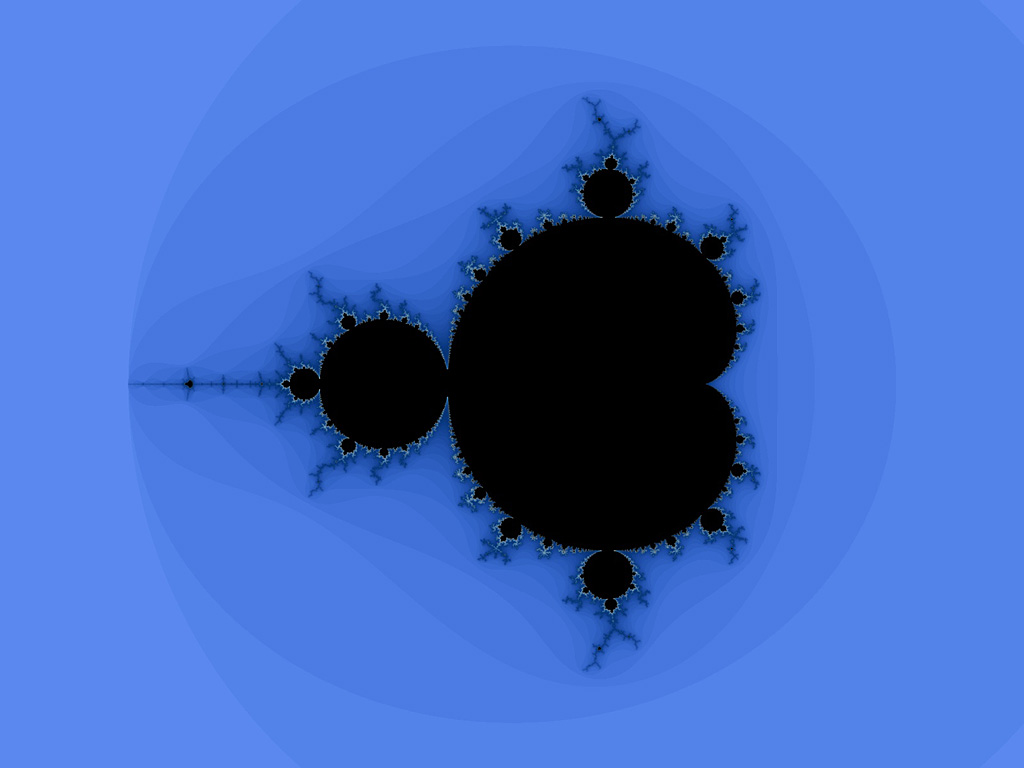
\includegraphics[width=8cm]{resources/mandelbrot.jpg}
        \label{fig:mandelbrot}
  }
  \subfloat[Ensemble de Julia] {
        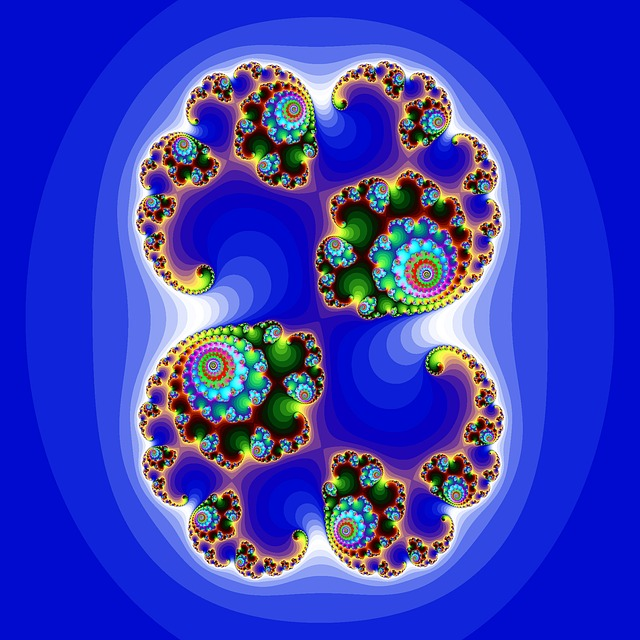
\includegraphics[width=8cm]{resources/julia.jpg}
        \label{fig:julia}
  }
  \caption{Figures géométriques générées à partir de fractales.}
\end{figure}

%% Les méthodes fractales utilisent les propriétés des formes fractales. Une forme fractale est un ensemble cohérent qui aura exactement la m\^eme structure quelque soit l'échelle utilisée. Dans notre projet, ces formes permettent deux choses :
%% \begin{itemize}
%% \item étant cohérente, une fractale représente un seul \og type de zone\fg\ ce qui permettent un rendu réaliste. Par exemple, une fractale représentant une montagne (hauteurs élevées) ne pourra pas présenter au milieu de sa structure un creux inattendu (hauteurs faibles) ;
%% \item le terrain généré garde la m\^eme apparence lorsque l'utilisateur utilise les fonctions de zoom. 
%% \end{itemize}

%% Certaines méthodes, dérivant des méthodes fractales, sont appelées \og multi-fractales\fg\ . Ces dernières offrent la possibilité de créer plusieurs entités fractales distinctes mais cohérentes. Le principe est de générer une première carte renseignant uniquement la hauteur de certains points puis d'intégrer les fractales adéquates selon la hauteur des points. Par exemple, admettons que nous travaillions sur cette carte d'élévations (pour mémoire, blanc = hauteur élevée, noir = hauteur faible) :
%% \begin{figure}[h!]
%%     \begin{center}
%%         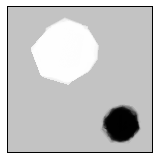
\includegraphics{resources/multi_fractales.png}
%%         \caption{Carte d'élévations factice}
%%         \label{multi-fractales}
%%     \end{center}
%% \end{figure}
%% nous pouvons nettement distinguer trois \og types de zones\fg\ distincts : une zone plane et homogène (grise), une zone élevée (blanche) et une zone basse (noire). Un algorithme multi-fractal appliqué à cette carte créerait trois fractales (une par zone) et des jonctions cohérentes entre les trois fractales. Ceci permet d'obtenir un terrain final cohérent sans être monotone.

Nous allons maintenant présenter les algorithmes des méthodes fractales suivantes : déplacement du point du milieu, diamant-carré et mouvement brownien fractionnaire.

\subsubsection{Déplacement du point du milieu (midpoint displacement)}
Cet algorithme a été introduit dans le livre \cite{Four82}, il prend en entrée
une carte d'élévation carrée vide et génère une élévation
pour chaque entrée de la grille.\\

L'algorithme commence par assigner une valeur aléatoire aux quatre cases
représentant les coins de la grille carrée.

Puis l'élévation du point du milieu de la grille est calculée en faisant
la moyenne des élévations des quatre coins auquel on ajoute une valeur
aléatoire.

Ensuite l'élévation des point des milieux des quatre côtés du carré est calculée
en faisant la moyenne des élévations des deux coins qui l'entourent.
\\

\`A l'issu de cette étape nous pouvons diviser la grille en quatre carrés
ayant tous une élévation assigné en leurs quatre coins.\\

On répète ensuite les deux étapes suivantes jusqu'à avoir rempli toutes les
cases de la grille :\\

\begin{itemize}
\item Pour chaque carré, calculer le point du milieu en faisant la moyenne
des élévations de ses quatre coins à laquelle est ajouté une valeur aléatoire.

\item Calculer le point du milieu de chaque côté du carré en faisant la moyenne
des élévation des deux coins qui l'entourent.\\
\end{itemize}

\`A chaque itération, on réduit l'amplitude de valeurs possibles pour
le nombre aléatoire généré.\\

La figure~\ref{fig:midpoint-displacement} illustre le déroulement de cet
algorithme pour une grille carrée (le principe est le même pour toutes les formes de grilles).

\begin{figure}[ht]
  \centering
  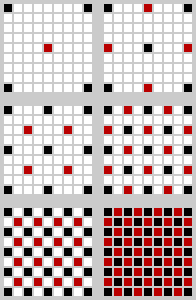
\includegraphics[width=4cm]{resources/midpoint-displacement.png}
  \caption{Déroulement de l'algorithme du déplacement du point du milieu (image
provenant de \cite{FractalTerrainGeneration}).}
  \label{fig:midpoint-displacement}
\end{figure}

\subsubsection{Diamant-carré}
L'algorithme diamond-square a été introduit pour la première fois dans le livre \cite{Four82}. Il s'agit d'une amélioration de l'algorithme de déplacement du point du
milieu. Il diffère de celui-ci dans le déroulement de l'étape du calcul des points
du milieu des côtés.\\

Lors ce cette étape, le point du milieu d'un côté n'est plus calculé seulement
en faisant la moyenne des élévations des deux coins qui l'entourent mais en faisant
la moyennes des élévations des quatre coin du losange englobant le point.\\

De plus une valeur aléatoire est ajoutée à cette moyenne.\\

Les figures~\ref{fig:side-midpoint} et~\ref{fig:side-diamond} illustrent la différence de calcul des points de milieux
des côtés entre l'algorithme de déplacement du point du milieu et celui du
diamant-carré.

\begin{figure}[h]
  \centering
  \subfloat[Algorithme de déplacement du point du milieu.] {
        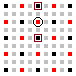
\includegraphics{resources/side-midpoint.png}
        \label{fig:side-midpoint}
  }
  \quad
  \subfloat[Algorithme du Diamant-carré.] {
        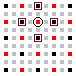
\includegraphics{resources/side-diamond.png}
        \label{fig:side-diamond}
  }
  \caption{Calcul du point du milieu d'un côté (images provenant de
    \cite{FractalTerrainGeneration}).}
\end{figure}



%% Cet algorithme a principalement été conçu pour recréer des montagnes artificielles sur un terrain déjà généré. L'idée est de partir d'un tableau carré à deux dimensions, la taille de ce tableau doit être un multiple de deux plus un (33x33, 65x65, 129x129, etc.). L'algorithme s'exécute en deux étapes.
%% \begin{itemize}
%% \item square : les quatre coins de la matrice sont fixés à la même valeur choisie aléatoirement. La valeur du centre du carré est ensuite calculée à partir de la moyenne des coins à laquelle on aura ajouté une valeur aléatoire ;
%% \item diamond : un diamant étant un losange dont le centre est la valeur initialement fixée, les extrémités du diamant de chaque centre sont moyennées.\\
%% Il faut alors diviser le pas et recommencer la manoeuvre.
%% \begin{figure}[h!]
%%     \begin{center}
%%         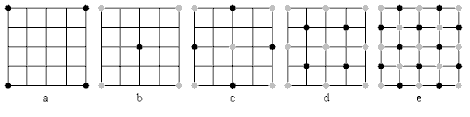
\includegraphics[width=10cm]{resources/square-diamond.png}
%%         \caption{Exemple Diamond-Square}
%%         \label{Diamond-Square}
%%     \end{center}
%% \end{figure}
%% \end{itemize}

\subsubsection{Fractional brownian motion (littéralement : mouvement brownien fractionnaire)}
Cet algorithme sert à appliquer N niveau de bruits sur chaque entrée d'une matrice d'élévation.
Le Fractional Brownian Motion prend en entrée :
\begin{itemize}
 \item un point de la matrice d'élévation;
 \item une méthode de bruits;
 \item une fréquence;
 \item une amplitude;
 \item un nombre d'octave correspondant aux nombres d'itérations successives d'un bruit;
 \item un degré de variation de la fréquence;
 \item un degré de variation de l'amplitude.
\end{itemize}
Il renvoi une valeur représentative de la hauteur du point traité.
\paragraph{}
Les entrées, citées précédemment, servent à configurer l'itération de bruits.
A chaque itération (dépendant du nombre d'octaves), plusieurs événements ont lieu :
\begin{itemize}
 \item mis-à-jour de la fréquence et de l'amplitude (\textit{via} le degré de variation de la fréquence et de l'amplitude);
 \item appel d'une méthode de bruit prennant plusieurs paramètres :
 \begin{itemize}
  \item le point à traiter;
  \item la fréquence;
  \item l'amplitude.
 \end{itemize}
 \item ajout de la valeur de sortie de la méthode de bruit aux précédents résultats.
\end{itemize}
Ainsi, cet algorithme consiste à itérer successivement la même méthode de bruit en faisant varier les paramètres d'entrées de ce dernier.
\paragraph{} 
Cet algorithme peut néanmoins ralentir la conception d'une carte d'élévation à cause du calcul des octaves (et donc des bruits) successifs.
Une description plus détaillé de l'algorithme est disponible dans l'article \cite{Mand68}.


\subsection{Les raffinements}
Les raffinements viennent modifier les hauteurs d'un terrain de façon à faire apparaître des détails liés à l'activité d'érosion, l'activité humaine, la présence de forêts, etc.
Ainsi ils apparaissent comme une sur-couche à ajouter après élaboration du terrain.\newline
Le document suivant \cite{Deus98} présente avec détail comment modéliser un écosystème sur un terrain. Un modèle d'érosion applicable sur la surface d'un terrain est décrit dans ce document \cite{Kell88}.

%%\chapter{Structures de données}

%% http://kiwi.atmos.colostate.edu/BUGS/geodesic/text.html
%% http://sydney.edu.au/engineering/it/~visual/valacon/pdf/papers/JNN06-SphericalSOM.pdf
%% http://www.smos.esa.int/ISEA/gdggs03.pdf
%% http://www.labri.fr/perso/fleury/courses/PdP/MondesVirtuels/terrain_generation/dggriddoc31.pdf
%% http://www.gamedev.net/topic/423908-making-a-mesh-from-a-geodesic-grid/
%% http://www.polycount.com/forum/showthread.php?t=96307

\section{Analyse des logiciels existant}
\subsection{Logiciels libres}
\subsubsection{LibNoise (figure~\ref{fig:libnoise})}
\label{ref:libnoise}

LibNoise~\cite{LibNoise} est une librairie portable et open-source développée en C++
permettant la génération de différents types de bruits cohérents, notamment
le bruit de Perlin (Perlin noise).

\begin{figure}[!ht]
    \begin{center}
        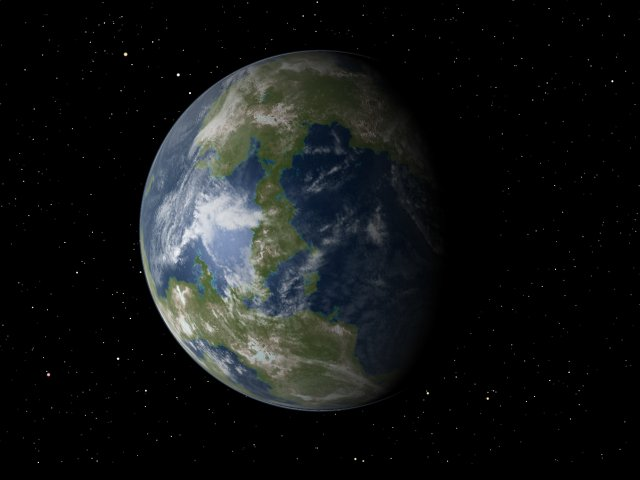
\includegraphics[width=10cm]{resources/libnoise.jpg}
        \caption{exemple de planète générée avec LibNoise rendue avec Celestia}
        \label{fig:libnoise}
    \end{center}
\end{figure}

\subsubsection{Fracplanet (figure~\ref{fig:fracplanet})}

Fracplanet~\cite{FracPlanet} est une application interactive permettant de visualiser et de générer aléatoirement des planètes et des terrains à l'aide de fractales.
Les objets générés peuvent être exportés dans des formats directement
utilisables par POV-Ray ou Blender.
Ce projet a été écrit en C++ et utilise QT et OpenGL.
Il est sous licence GPL.

\begin{figure}[!ht]
    \begin{center}
        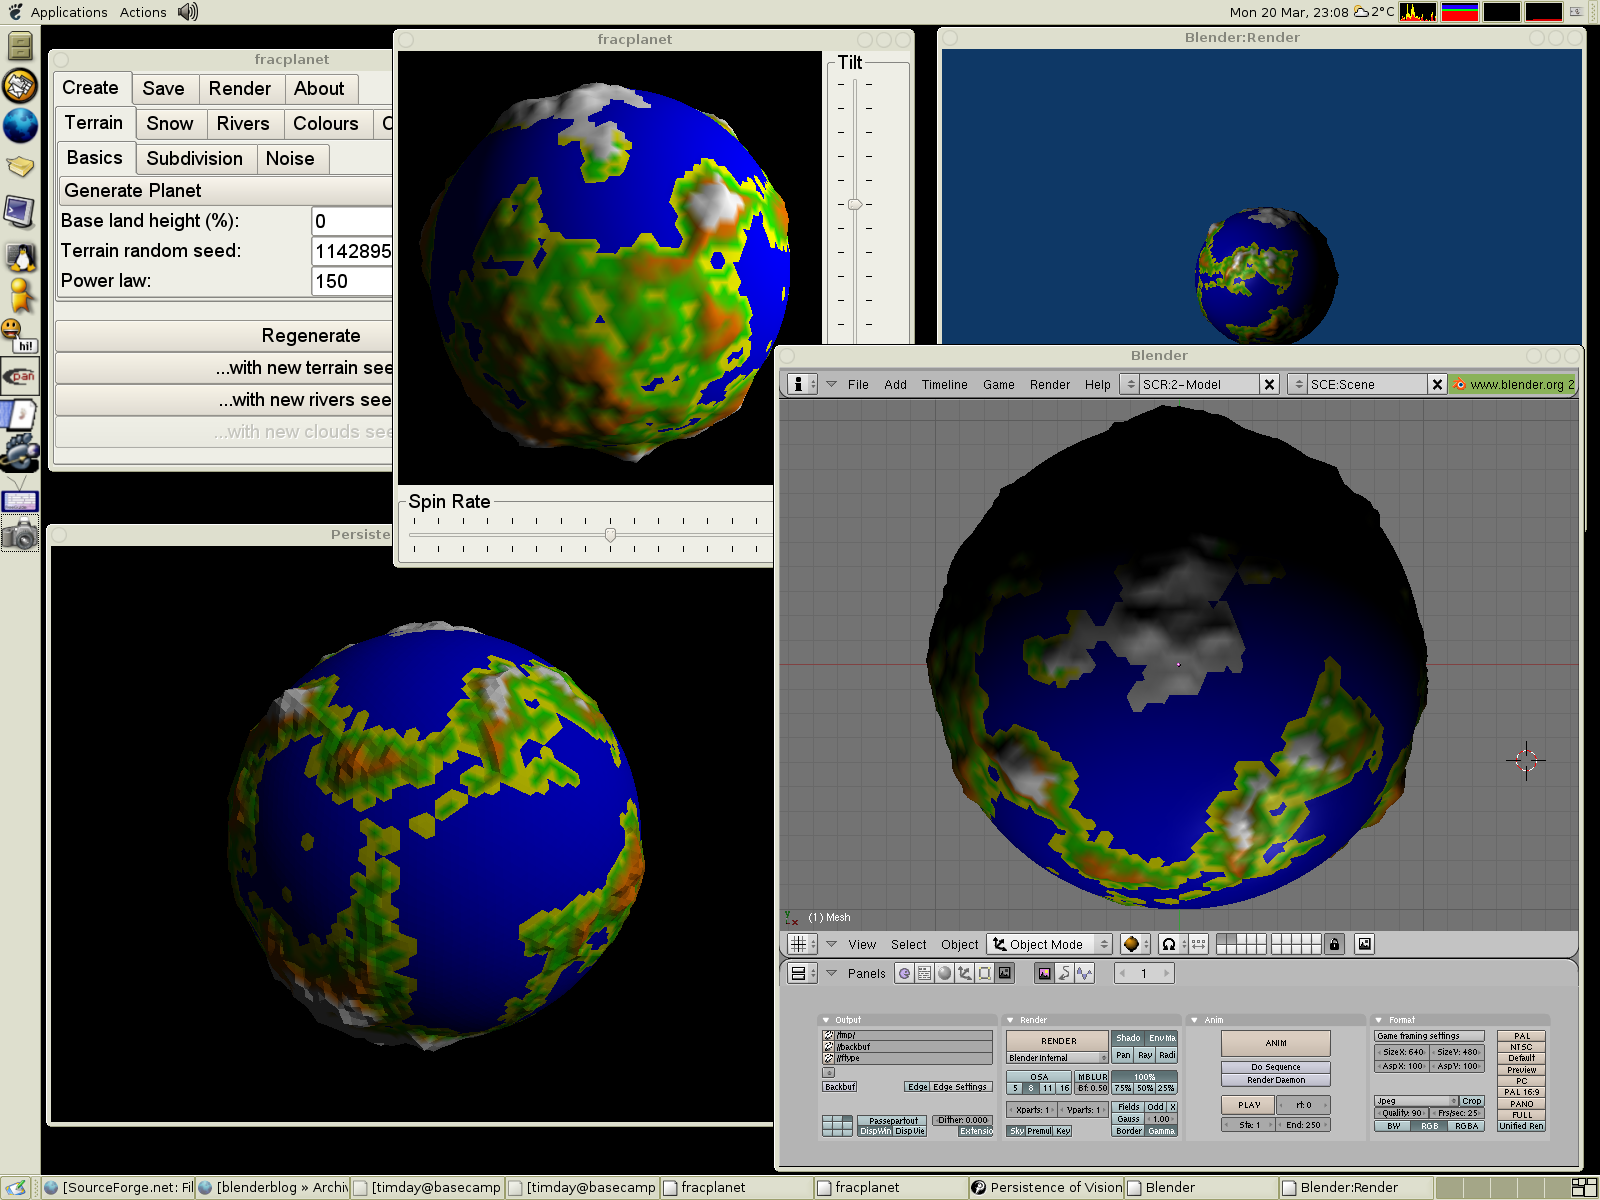
\includegraphics[width=10cm]{resources/fracplanet.png}
        \caption{capture d'écran de FracPlanet}
        \label{fig:fracplanet}
    \end{center}
\end{figure}

\subsubsection{TerraJ (figure~\ref{fig:terraj})}
TerraJ~\cite{TerraJ} est une collection de programmes de génération de terrains fractals et de systèmes solaires (dont Fracplanet) portés du C/C++ vers Java sous licence GPL.

\begin{figure}[!ht]
    \begin{center}
        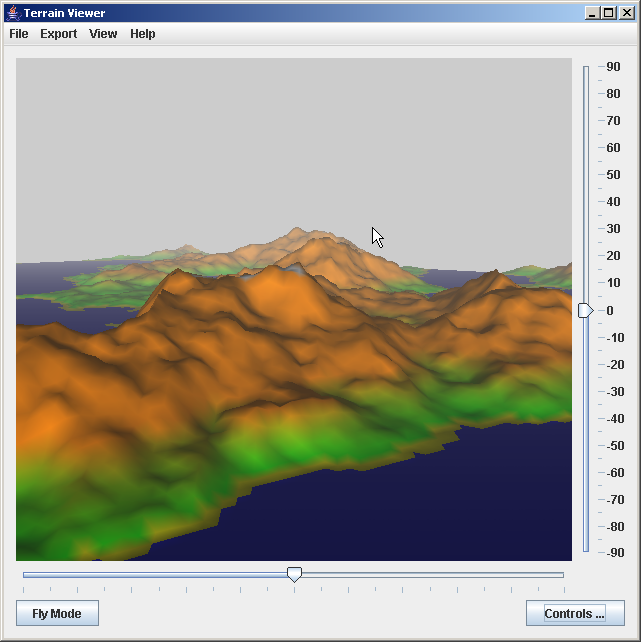
\includegraphics[width=10cm]{resources/terraj.png}
        \caption{capture d'écran de TerraJ}
        \label{fig:terraj}
    \end{center}
\end{figure}

\subsubsection{Terrain.dk (figure~\ref{fig:terrain_dk})}
Le but de ce projet~\cite{largeDetTerrainsURL} open source est de permettre de
visualiser un terrain vaste et détaillé. Les développeurs se sont basé sur deux algorithmes
d'affichages de niveau de détail. Ils utilise "the chunked quadtree structure"
crée par Ulrich ~\cite{Ulrich2002}, mais avec le processus de simplication du
Dr Boer ~\cite{citeulike:623420}.

\begin{figure}[!ht]
    \begin{center}
        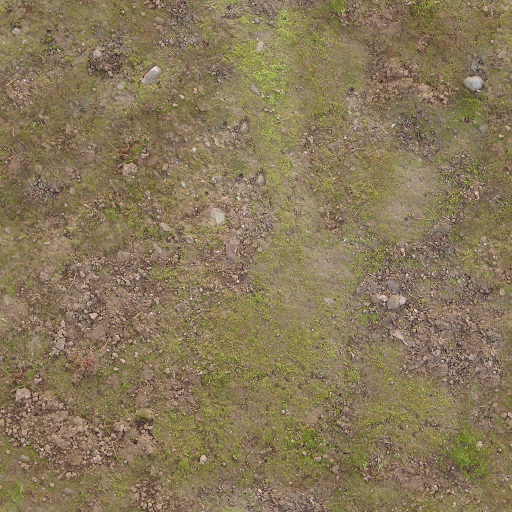
\includegraphics[width=10cm]{resources/terraindk.png}
        \caption{capture d'écran de Terrain.dk}
        \label{fig:terrain_dk}
    \end{center}
\end{figure}

\subsubsection{Irrlicht 3D Engine (figure~\ref{fig:irrlicht})}
Irrlicht 3D Engine ~\cite{irrlicht} est un logiciel libre sous licence zlib, donc compatible avec notre projet. Ce moteur graphique développé par Nikolaus Gebhardt et al. est utilisé dans divers domaines comme la visualisation de planète où les jeux vidéo.
\begin{figure}[!ht]
    \begin{center}
        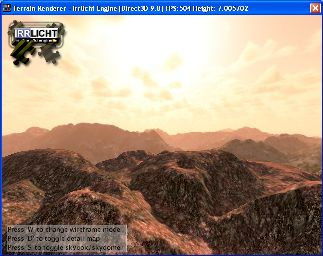
\includegraphics[width=10cm]{resources/irrlicht.jpg}
        \caption{capture d'écran de Irrlicht}
        \label{fig:irrlicht}
    \end{center}
\end{figure}

\newpage
\subsection{Logiciels propriétaires}
\subsubsection{Terragen (figure~\ref{fig:terragen})}
Terragen~\cite{Terragen} est un générateur de terrain très populaire écrit en C++  pour Windows et Mac OS X développé par Planet Side. Il a notamment été utilisé pour la réalisation d'effets spéciaux dans les films : Gatsby le Magnifique (2013), Man of Steel (2013), Tron l'héritage (2010) et bien d'autres.

Il s'agit d'un logiciel propriétaire payant mais il existe aussi une version gratuite aux fonctionnalités limitées pour un usage non commerciale.

\begin{figure}[!ht]
    \begin{center}
        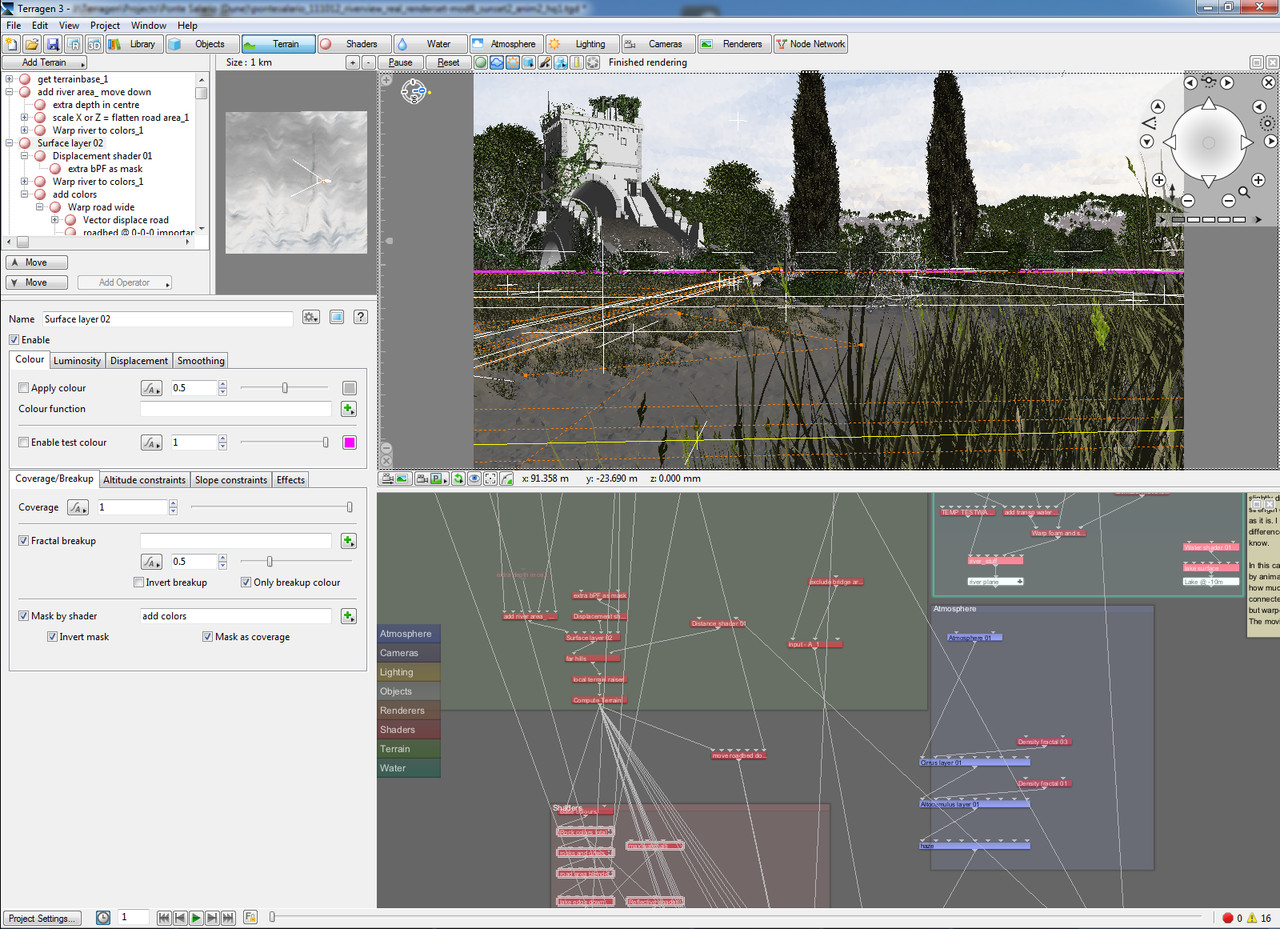
\includegraphics[width=10cm]{resources/terragen.jpg}
        \caption{capture d'écran de Terragen}
        \label{fig:terragen}
    \end{center}
\end{figure}

\subsubsection{MojoWorld (figure~\ref{fig:mojoworld})}
MojoWorld~\cite{Mojoworld} est un générateur de planète propriétaire pour Windows et Mac OS X
commercialisé par Pandromeda Inc.
Il a été crée à l'origine par Ken Musgrave, l'auteur du livre~\cite{Eber02}.

\begin{figure}[!ht]
    \begin{center}
        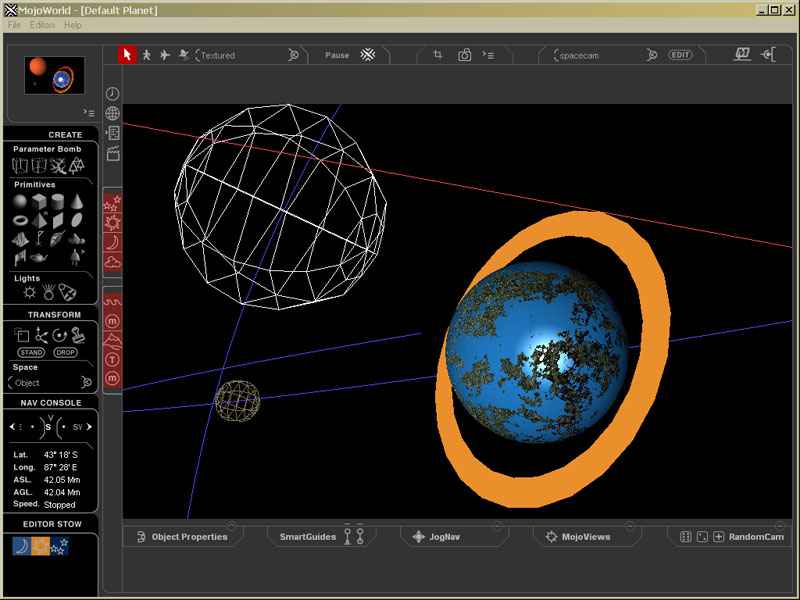
\includegraphics[width=10cm]{resources/mojoworld.jpg}
        \caption{capture d'écran de MojoWorld}
        \label{fig:mojoworld}
    \end{center}
\end{figure}

\subsubsection{Vue (figure~\ref{fig:vue})}
Vue~\cite{Vue} est un générateur de paysages propriétaire pour Windows et Mac OS X.
Il est utilisé pour la création, l'animation et la visualisation d'environnements 3d naturels. Il a été utilisé pour réaliser des effets spéciaux dans de
nombreux films tels que Indiana Jones et le Royaume du crâne de cristal (2008) et Pirates des Caraïbes : Le Secret du coffre maudit (2006).
\begin{figure}[!ht]
    \begin{center}
        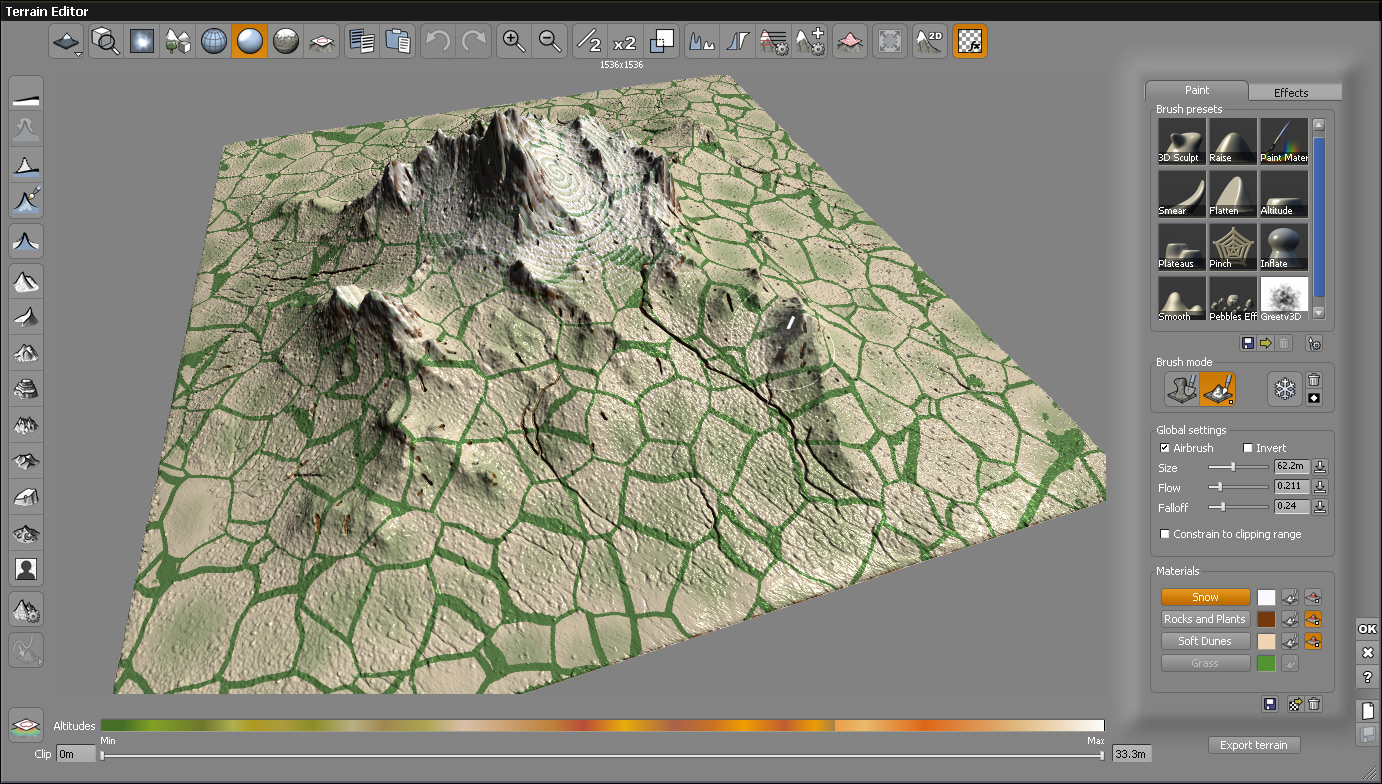
\includegraphics[width=10cm]{resources/vue.jpg}
        \caption{capture d'écran de Vue}
        \label{fig:vue}
    \end{center}
\end{figure}

\subsubsection{Grome (figure~\ref{fig:grome})}
Grome~\cite{Grome} est un logiciel propriétaire de modélisation 3D pour Windows utilisé dans l'industrie des jeux vidéos. Il est développé par Quad Sofware et permet
notamment la génération procédurale de terrain à l'aide de fractales.
\begin{figure}[!ht]
    \begin{center}
        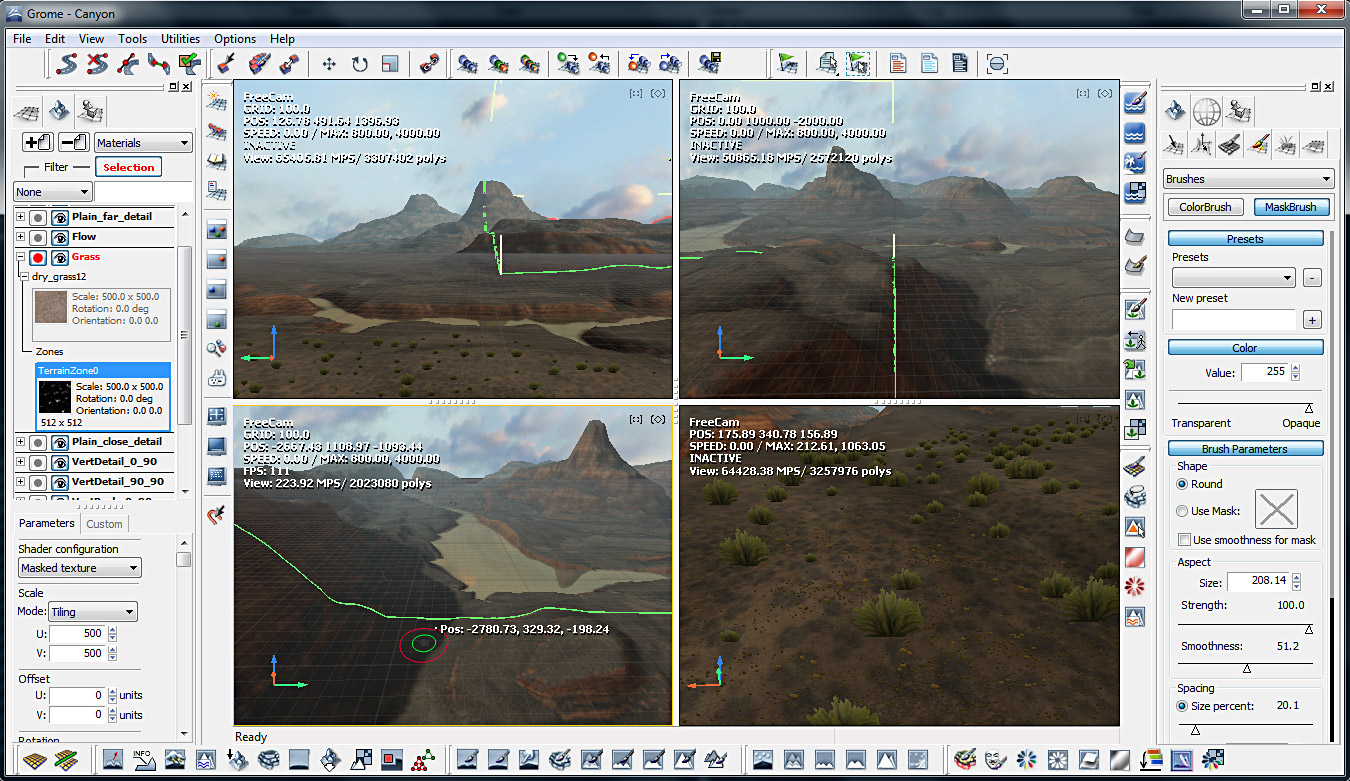
\includegraphics[width=10cm]{resources/grome.jpg}
        \caption{capture d'écran de Grome}
        \label{fig:grome}
    \end{center}
\end{figure}
